\ylDisplay{Veepüstol} % Ülesande nimi
{Valter Kiisk} % Autor
{lõppvoor} % Voor
{2006} % Aasta
{G 4} % Ülesande nr.
{5} % Raskustase
{
% Teema: Vedelike-mehaanika
\ifStatement
Veepüstoliga (vt joonist) tekitatakse veejuga, surudes vett läbi kitsa silindrilise suudme, mille sisediameeter on $d_2 = \SI{1}{mm}$. Päästik on ühendatud kolviga, mis saab tihedalt liikuda silindrilises torus diameetriga $d_1 = \SI{1}{cm}$. Oletagem, et sõrmed suruvad päästikule jõuga $F = \SI{20}{N}$ (jõu rakenduspunkt ja suund on näidatud joonisel). Kui suure kiirusega väljub veejuga püstolist? Vee liikumise võib lugeda laminaarseks, vee viskoossust ja püstoli liikuvatele osadele mõjuvaid hõõrdejõude võib ignoreerida. Vee tihedus on $\rho = \SI{1000}{kg/m^3}$

\begin{center}
	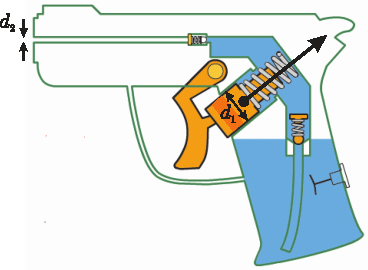
\includegraphics[width=0.6\linewidth]{2006-v3g-04-yl}
\end{center}
\fi


\ifHint
Kolbile mõjuv jõud tekitab kolvi sees lisarõhu $F/S$. Kuna tegu on laminaarse vooga, kehtib Bernoulli seadus. Alternatiivselt võib rakendada energia jäävust kolvi ees ja suudme juures.
\fi


\ifSolution
Kuna me ei arvesta dissipatiivseid effekte, siis peab kehtima mehaanilise energia jäävus. Liikugu kolb jõu $F$ toimel kiirusega $v_1$ ja olgu vee kiirus suudmes $v_2$. Kuna vee koguruumala ei muutu, siis $v_1S_1 = v_2S_2$. Ajavahemiku $t$ vältel
läbib kolb vahemaa $x = v_1t$ tehes tööd $A = F x$. Vaatame, milline on sellele liikumisele vastav vee summaarne kineetilise energia muut. Ühelt poolt kolvi eest \enquote{kaob ära} veehulk $m = S_1x\rho$, mille kiirus oli $v_1$, teiselt poolt ilmub suudmesse sama kogus vett liikudes kiirusega $v_2$. Energia jäävus annab
\[
A+\frac{m v_{1}^{2}}{2}=\frac{m v_{2}^{2}}{2}
\]
ehk peale asendamist ja $v_1$ elimineerimist
\[
\frac{F}{S_{1}}+\frac{\rho v_{2}^{2}}{2} \frac{S_{2}^{2}}{S_{1}^{2}}=\frac{\rho v_{2}^{2}}{2}.
\]
Aga $d_2 \ll d_1$ ja $S \propto d^2$, seega ammugi $S_2^2 \ll S_1^2$ ning teise liikme vasakul pool võrdusmärki võib ära jätta. Avaldame $v_2$:
\[
v_{2}=\frac{1}{d_{1}} \sqrt{\frac{8 F}{\pi \rho}} \approx \SI{22,6}{m/s}.
\]

\emph{Märkus}. Ülesande oleks saanud lahendada ka kiiremat teed pidi lähtudes Bernoulli seadusest
\[
p+\frac{\rho v^{2}}{2}=\const,
\]
mille me lahendamise käigus sisuliselt tuletasime.
\fi
}